% \section{Motivation}

\section{Guide to use HCPC}
The tool can be used in two ways. First, a developer new to the code-base can load the abstraction tree which start with the root node. In the right side panel, for each node the number of execution paths, a brief natural text summary, and few frequent execution patterns are presented. Therefore, the developer can start first by observing summary, patterns of the root node. Now, the child nodes of the root node can be expanded and  similarly explored by observing corresponding node summary and patterns. The developer can continue this way according to their need to get acquainted with the coda-base behavior and high-level concepts in the code-base.

Second, a new contributor to a open source project can utilize the tool to understand high-level concepts related to a specific method. Developers first start from looking to open issues of a repository to find something work on. The issues are natural text description which provides information regarding a bug or a feature enhancement request. Developers can identify few keywords and use our tool to find matching methods relevant to the keywords. Next, a specific method can be selected to highlight relevant nodes in the tree. The difference between the first approach here is developers will be able to browse the tree with focus to the selected method. The node titles relevant to selected method will be highlighted so that the developer can expand their child nodes. By this way, the developer can start from the high-level concept to low-level source code related concepts for a specific method. By iterating this process, the developer can grasp high-level domain knowledge (with comment summary and IR techniques on function names) alongside insight into program execution scenarios which decreases the overhead due to lack of domain knowledge in the code-base. 

\section{Graphical demo of the tool} 
We have picked \emph{jupyter-client}\footnote{https://github.com/jupyter/jupyter\_client} as the subject system to show how the tool can be used following the two above mentioned techniques. To discuss the effectiveness of our tool using \emph{jupyter-client}, first we will discuss high level functionalities of \emph{jupyter-client} from their documentation. Later, we will present the information provided by our tool and discuss whether our tool provides similar or more information to comprehend the \emph{jupyter-client} project. \emph{jupyter-client} has three components. First, \emph{kernelspec} deals with specify different type of kernels from predefined files. Second, kernel manager which is responsible for start, stop and signaling kernels for different scenarios. Third, kernel client which is responsible for communicating with kernels for code execution and other tasks \footnote{https://jupyter-client.readthedocs.io/en/stable/index.html}. From the above components we can get an abstract idea of the features of \emph{jupyter-client}. Now, we will discuss the high-level features suggested by HCPC tool. Below we have listed few high-level features of the \emph{jupyter-client} project. The features are found by expanding the tree to three depth. More specific features are possible to get by diving deep into the tree.

\begin{figure*}[h]
  \centering
  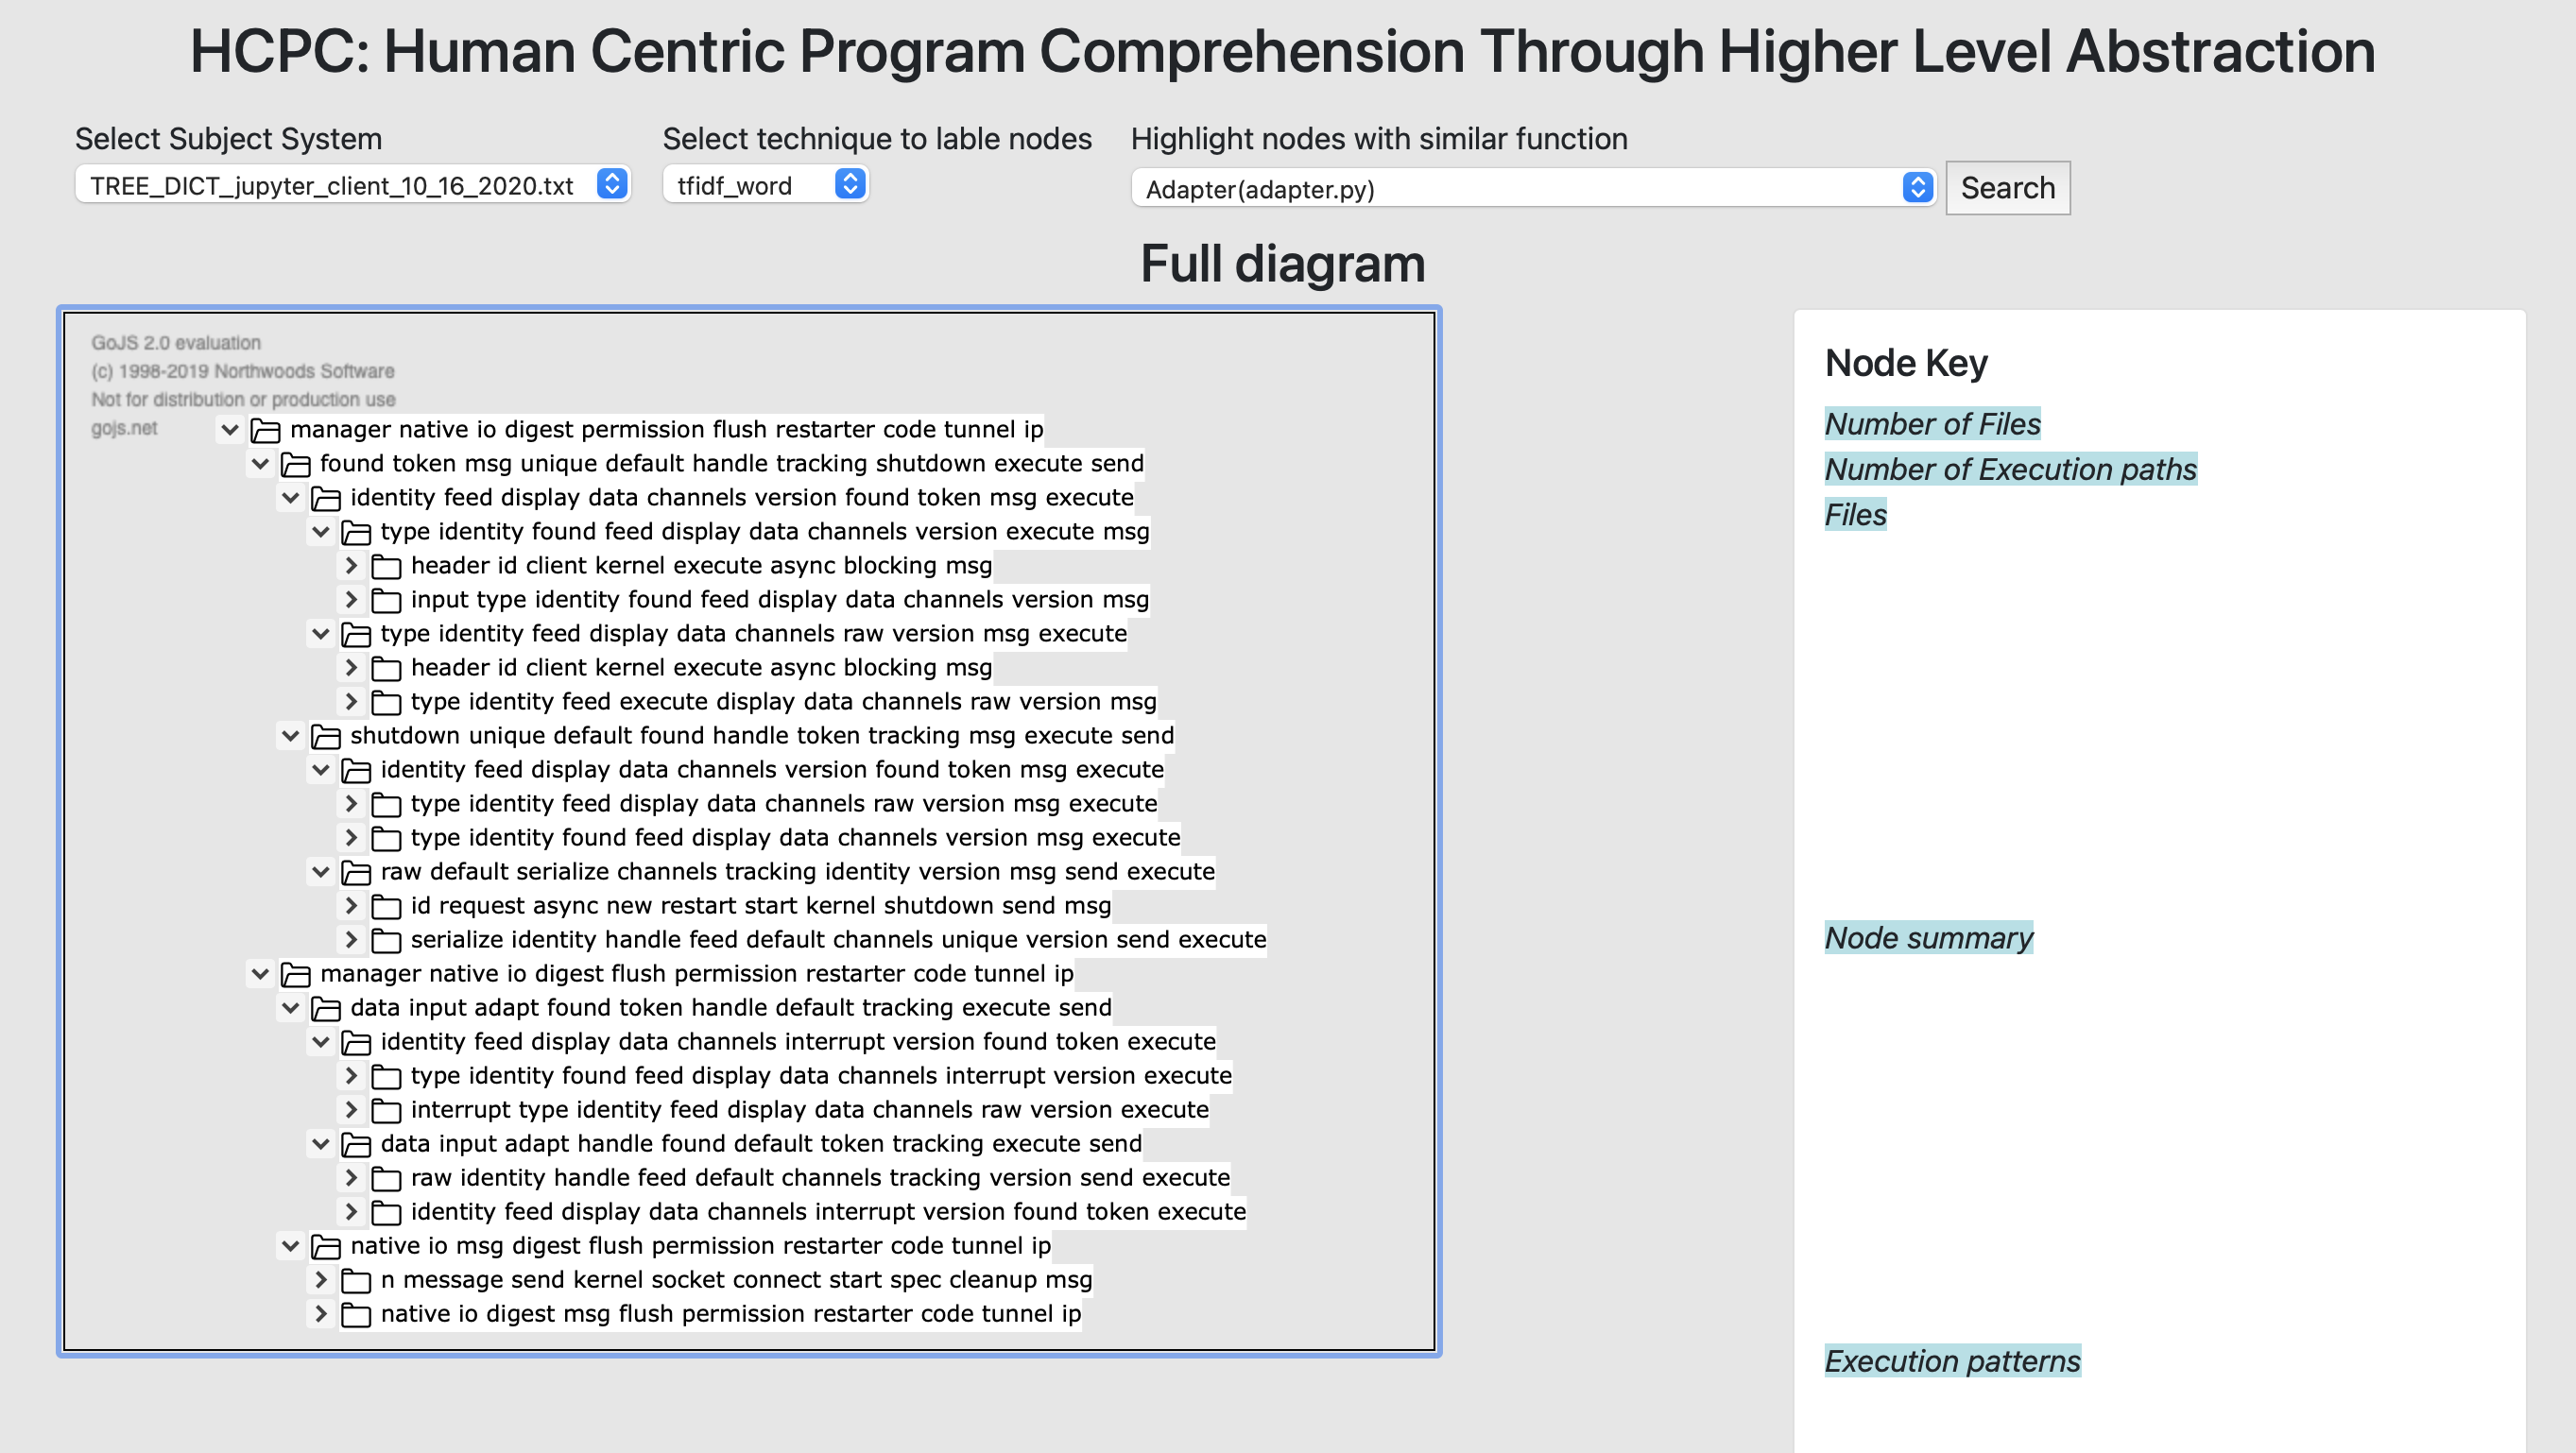
\includegraphics[width=\columnwidth]{figures/hla3/tool_overview_jupyter.png}
  \caption{HCPC tool overview for jupyter\_client project }~\label{fig:tool_overview_jupyter_client}
\end{figure*}

\begin{itemize}
    \item Request kernel info. Request comm info. Tab complete text in the kernel's namespace. Get metadata information about an object in the kernel's namespace. Ask the kernel whether some code is complete and ready to execute.
    \item Forgets randomly assigned port numbers and cleans up the connection file. Restarts a kernel with the arguments that were used to launch it. Write connection info to JSON dict in self.connection\_file. Restarts a kernel with the arguments that were used to launch it.
    \item Request kernel info. Given a message or header, return the header. Request comm info. Tab complete text in the kernel's namespace. wrapper for doing common steps for validating an execution request. Pass a message to the ZMQ socket to send. message format.
    \item Send a shutdown request via control channel. Attempts to stop the kernel process cleanly. Restarts a kernel with the arguments that were used to launch it.
\end{itemize}

From the above text blocks, we can understand that \emph{jupyter-client} is relevant to working with kernels, it uses ZMQ socket to communicate with kernels, and work with kernel information. 

Next, it is possible to browse the tree by focusing on a specific method. In figure \ref{fig:tool_shutdown_all}, we can see the nodes in the tree are marked to indicate they are relevant to shutdown\_all method. Developers can investigate the nodes marked to understand relevant features of shutdown\_all method. 

\begin{figure*}[h]
  \centering
  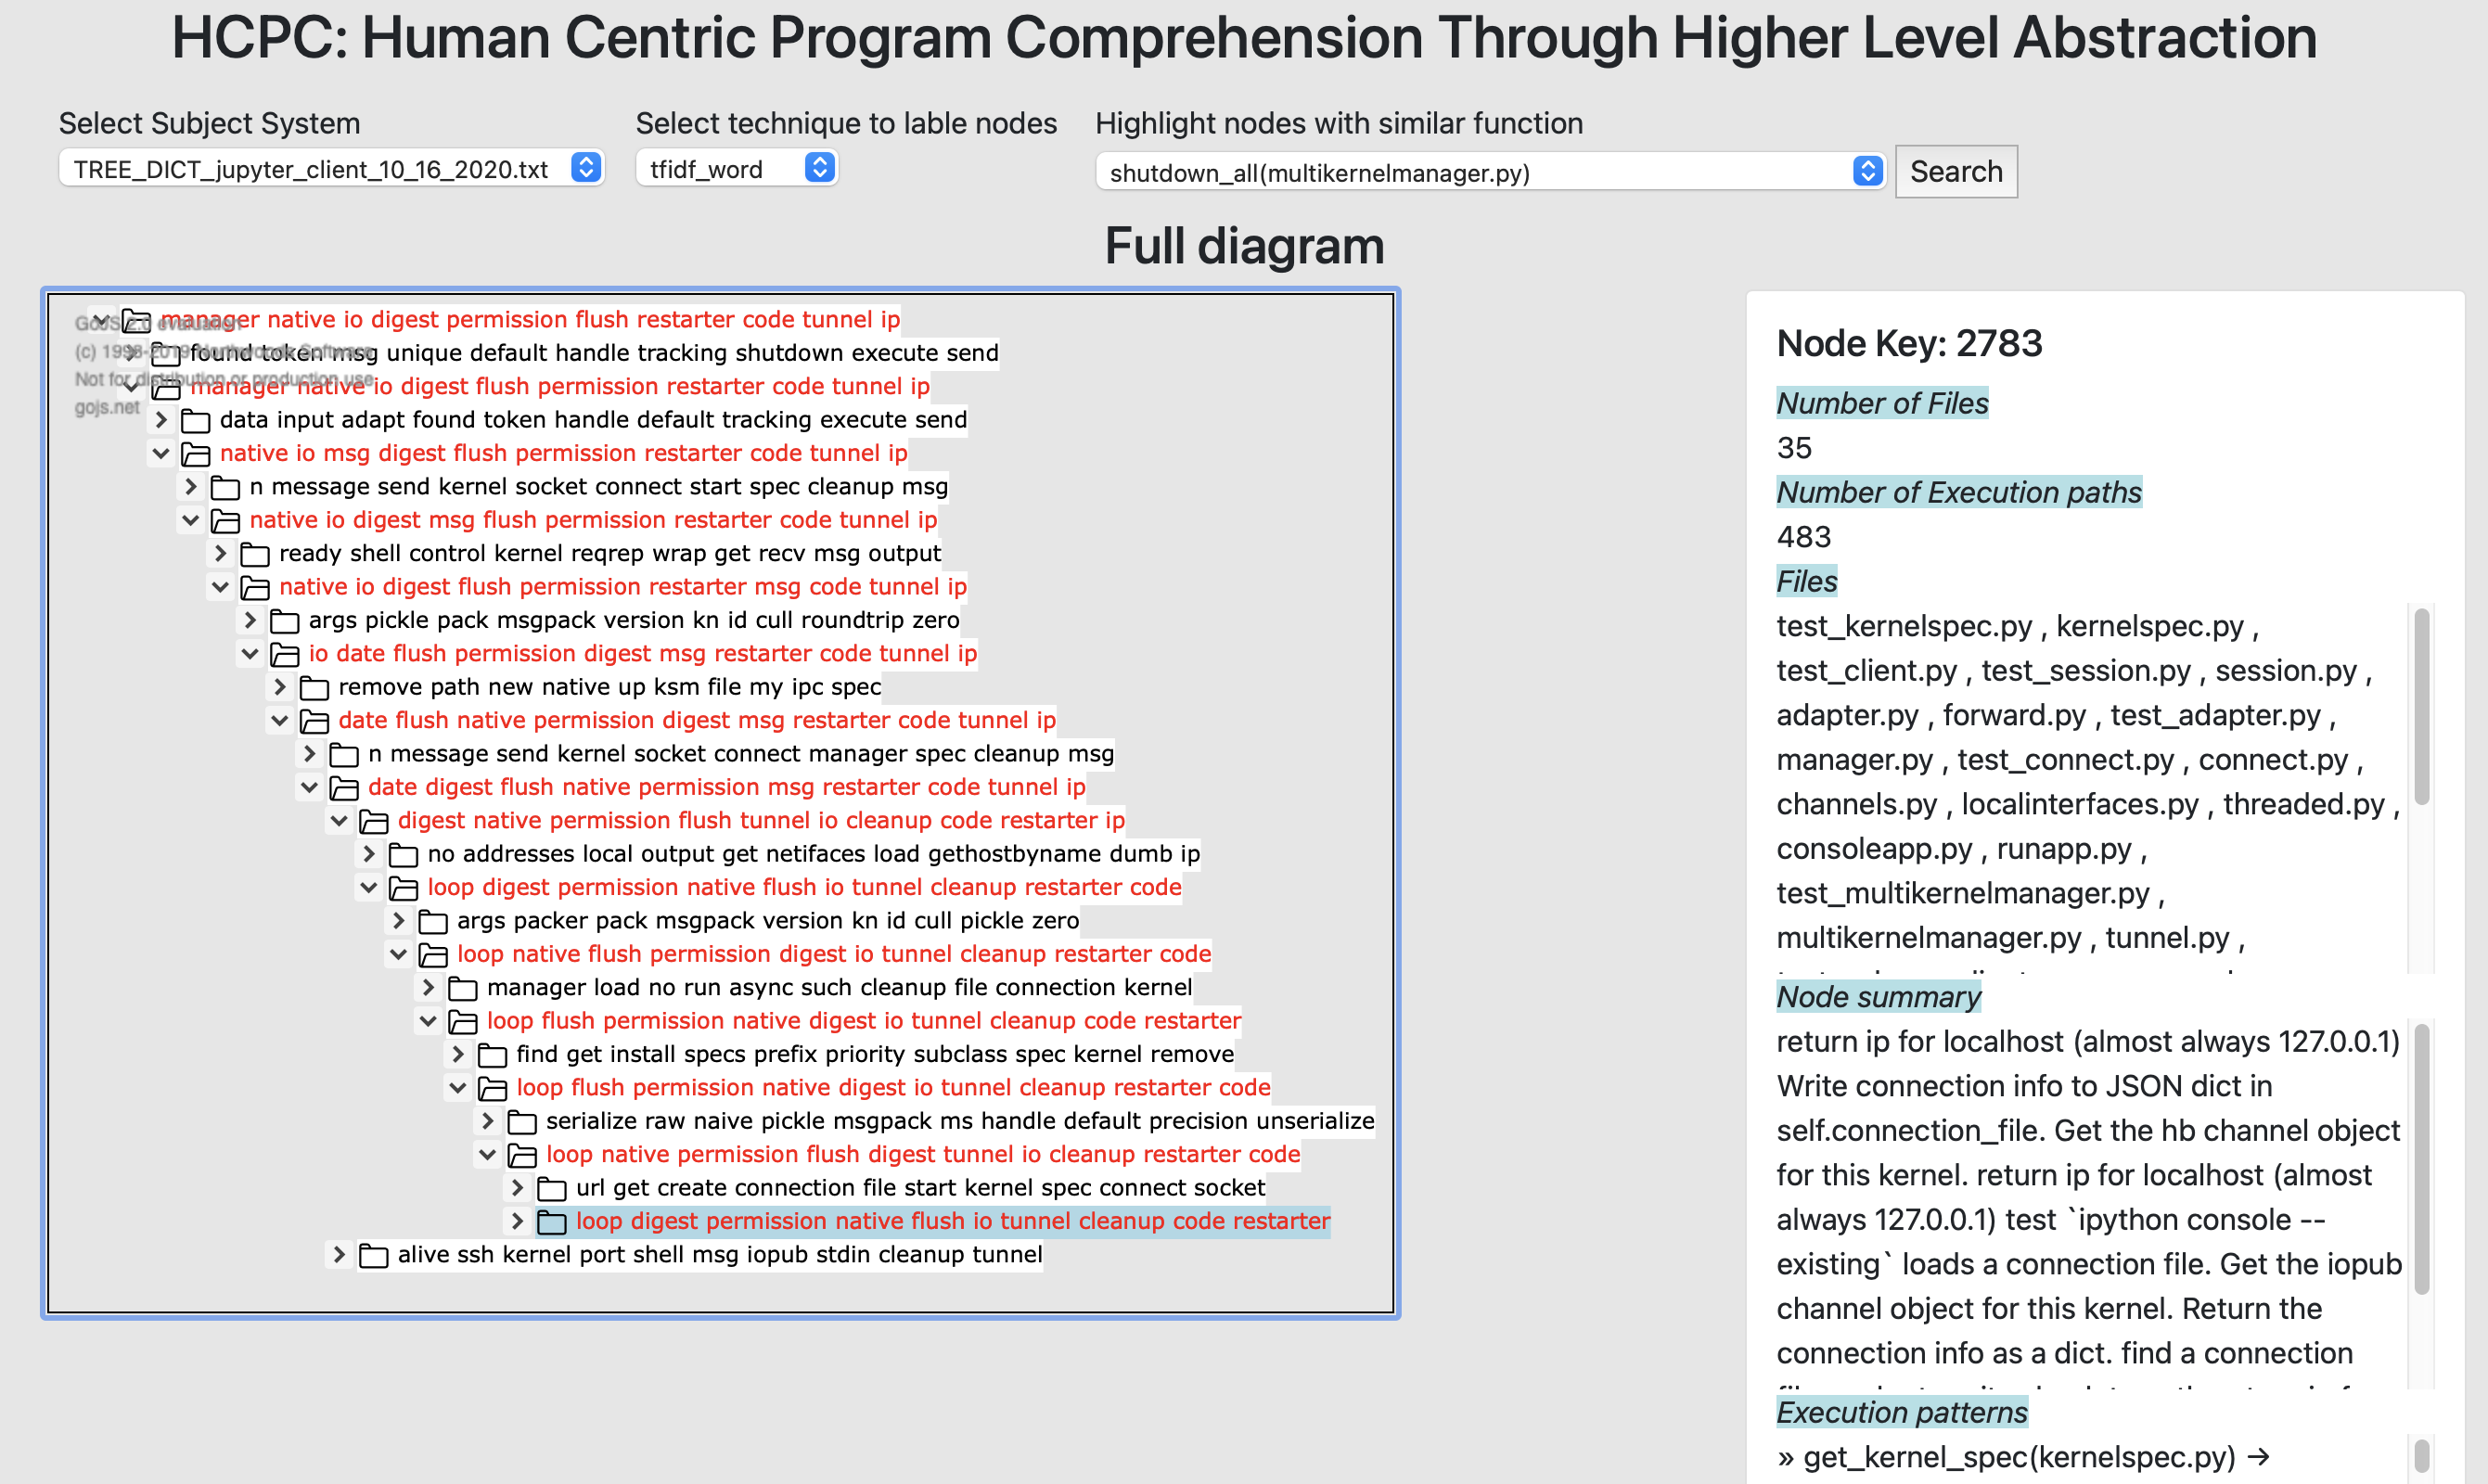
\includegraphics[width=\columnwidth]{figures/hla3/tool_shutdown_all.png}
  \caption{HCPC tool when focusing to find features related to shutdown\_all method }~\label{fig:tool_shutdown_all}
\end{figure*}


\begin{itemize}
    \item check that a kernel id is valid. Interrupts the kernel by sending it a signal. Wait for kernel shutdown, then kill process if it doesn't shutdown. Shutdown all kernels. Sends a signal to the process group of the kernel (this. Restarts a kernel with the arguments that were used to launch it. Attempts to stop the kernel process cleanly. Get the single KernelManager object for a kernel by its uuid.
    \item Get the hb channel object for this kernel. Get the stdin channel object for this kernel. Stops all the running channels for this kernel. Get the iopub channel object for this kernel. Get the control channel object for this kernel. Get the shell channel object for this kernel.
    
\end{itemize}

From above information provided by the tool, we can know how the shutdown\_all method works. Also we know that kernel object has different kind of channels for communication such as iopub, stdin.  
